\documentclass[10pt, xcolor=dvipsnames]{beamer}

\usetheme{metropolis}
\usepackage[utf8]{inputenc}
\usepackage[english]{babel}
\usepackage{ragged2e}
\usepackage{bbding}
%\usepackage{enumitem}
\usepackage{mathtools}
\usepackage{indentfirst}
\usepackage{graphicx}
\usepackage{float}
\usepackage{hyperref}
\usepackage{mathtools}
\usepackage{preview}
\usepackage{xcolor}
\usepackage{color}
\usepackage{listings}
\usepackage{float}
\usepackage[caption = false]{subfig}
\usepackage{pdfpages}
\usepackage{multirow}
\usepackage{array}
\usepackage{makecell}
\usepackage{bm}
\usepackage{caption}
\usepackage{cancel}
\usepackage{anyfontsize}
\usepackage{etoolbox}
\usepackage{mathtools}

\usepackage[flushleft]{threeparttable}
\usepackage{booktabs}
\usepackage{caption}
\usepackage{adjustbox}
\usepackage{appendixnumberbeamer}
\usepackage{pifont}
\usepackage{amsmath}
\usepackage{amssymb}
\usepackage[percent]{overpic}

%\usepackage{biblatex}
\usepackage[backend=biber,
style=authoryear,
citestyle=authoryear]{biblatex} 
\addbibresource{latex/bibliography.bib}

\setbeamercolor{titlelike}{parent=structure}
\definecolor{UBCblue}{rgb}{0.04706, 0.13725, 0.32}
\colorlet{UBCblue2}{UBCblue!70!white}
\usecolortheme[named=UBCblue]{structure}

\makeatletter
\setbeamertemplate{footline}
{
  \leavevmode%
  \hbox{%
  \begin{beamercolorbox}[wd=.4\paperwidth,ht=2.25ex,dp=1ex,center]{author in head/foot}%
    \usebeamerfont{author in head/foot} \insertshortauthor %\hspace*{1em}(\insertshortinstitute)
  \end{beamercolorbox}%
  \begin{beamercolorbox}[wd=.5\paperwidth,ht=2.25ex,dp=1ex,center]{title in head/foot}%
    \usebeamerfont{title in head/foot} \insertshorttitle
  \end{beamercolorbox}%
  \begin{beamercolorbox}[wd=.1\paperwidth,ht=2.25ex,dp=1ex,center]{date in head/foot}%
    \usebeamerfont{date in head/foot}
    \insertframenumber{} / \inserttotalframenumber\hspace*{2ex} 
  \end{beamercolorbox}}%
  \vskip0pt%
}
\makeatother

\renewcommand{\arraystretch}{1.2}
\renewcommand{\raggedright}{\leftskip=0pt \rightskip=0pt plus 0cm}
\newcolumntype{C}[1]{>{\centering\let\newline\\\arraybackslash\hspace{0pt}}m{#1}}

\hypersetup{
    colorlinks=true,
    linkcolor=UBCblue,
    citecolor=UBCblue,
    filecolor=magenta,      
    urlcolor=blue,
    allcolors=.
}

\setbeamercolor{button}{bg=UBCblue2,fg=white}
\newcommand\fnote[1]{\captionsetup{font=tiny}\caption*{#1}}
\newcommand\fnotev[1]{\captionsetup{font=scriptsize}\caption*{#1}}
\def\house{\hbox{\kern3pt \vbox to13pt{}% 
   \pdfliteral{q 0 0 m 0 5 l 5 10 l 10 5 l 10 0 l 7 0 l 7 5 l 3 5 l 3 0 l f
               1 j 1 J -2 5 m 5 12 l 12 5 l S Q }%
   \kern 13pt}}
\setbeamertemplate{caption}[numbered]
\setbeamertemplate{itemize item}{\Tiny \house}
\metroset{progressbar=frametitle,numbering=fraction}
% %\justifying
% \urlstyle{same}
%\usefonttheme{serif}

%\usefonttheme{serif}

%------------------------
%------------------------

\date{}

%------------------------
%------------------------
%----------------------------------------------------------------------------------------
%	TITLE PAGE
%----------------------------------------------------------------------------------------------------------------
%------------------------

\title[Landlord Responses to Changes in Tenant Protections]{Are Slumlords Necessary: \\Landlord Responses to Changes in Tenant Protections} % The short title appears at the bottom of every slide, the full title is only on the title page
\author[Joe Fish]{Joe Fish}


\begin{document}

\begin{frame}
\titlepage % Print the title page as the first slide
\end{frame}

\begin{frame}{Motivation}
    \begin{enumerate}
        \item About 80\% of low income renters live in private market units \parencite{jchs_2024, nhpd2024profiles}
        \pause
        \item Low income landlords are both more punitive (lower threshold to evict) and more profitable \parencite{Desmond_2019, Eisfeldt_2015,Damen_2025}
        \item Evictions have large personal and social cost \parencite{desmond-evicted,humphries2025, collison-et-al-2023}
        \begin{itemize}
            \item Suggests room to regulate the worst landlords
        \end{itemize}
        \pause
        \item At the same time, given reliance on private market and lack of funds for subsidized housing, optimal regulation has to be careful about inducing landlord exit
        \begin{itemize}
            \item Optimal regulation requires the distribution of exit/upgrade options across landlords
        \end{itemize}
    \end{enumerate}

\end{frame}


\begin{frame}{Questions of Interest}
    \begin{itemize}
        \item How do landlords respond to changes in tenant protections?
        \begin{itemize}
           \item Case study of overhaul of eviction process in Philadelphia, PA
        \end{itemize}
         \item How do landlord responses vary by market position, outside option, etc.?
         \item Given landlord response function, what does optimal regulation look like?
    \end{itemize}
\end{frame}

\begin{frame}{This Presentation}
    \begin{enumerate}
        \item Background on Philadelphia rental market, eviction diversion program, and right to counsel
        \item Toy model of landlord response to change in tenant protections
        \item Nested logit of market segmentation
        \item Reduced form evidence of changes in landlord behavior (pricing, maintenance)
    \end{enumerate}
    
\end{frame}

\begin{frame}{Existing Literature}
    \textbf{Rent Control}
    \begin{itemize}
        \item Studies on price effects \cite{diamond-2019, Jofre_Monseny_2023, Kholodilin_2024}
        \item Studies on housing quality \cite{Gyourko_1990 }
    \end{itemize}
    \textbf{Tenant Protections}
    \begin{itemize}
        \item \cite{humphries-2024}: Looks at how landlords respond to a change in tenant protections in NYC; finds price pass through onto tenants
        \item \cite{abramson_2021, Asquith_2019, Corbae_2024}
    \end{itemize}
    
\end{frame}


\section{Data}

\begin{frame}{Data}
\textbf{Eviction Data}
    \begin{itemize}
        \item Universe of Eviction Records from 2006-2025
        \begin{itemize}
            \item Contain \textbf{contract rents} as well case information (address, amount owed, plaintiff / defendant name, etc.)
            \item Cases are filtered to non-commercial and non-housing authority
        \end{itemize}
    \end{itemize}
\pause
\textbf{Rental listing data from Altos (2011-2023)}
\begin{itemize}
    \item Unit level rental listings with information on amenities, beds, baths, etc.
\end{itemize}
\textbf{ Rental Registry}
\begin{itemize}
    \item Covers near-universe of rental listings
    \item Importantly, landlords need to be on the rental listing to file evictions
\end{itemize}
\textbf{Address History Data from Infutor}
    \pause
Why this is important:\\
    \begin{itemize}
        \item This will be one of the few papers to study the low income rental market because data are so sparse 
    \end{itemize}
\end{frame}

\begin{frame}{Distribution of Rent Prices by Data Source}
Commercially available rental datasets (\textcolor{red}{altos}) don't cover the low income rental market\\
    \begin{figure}
        \centering
        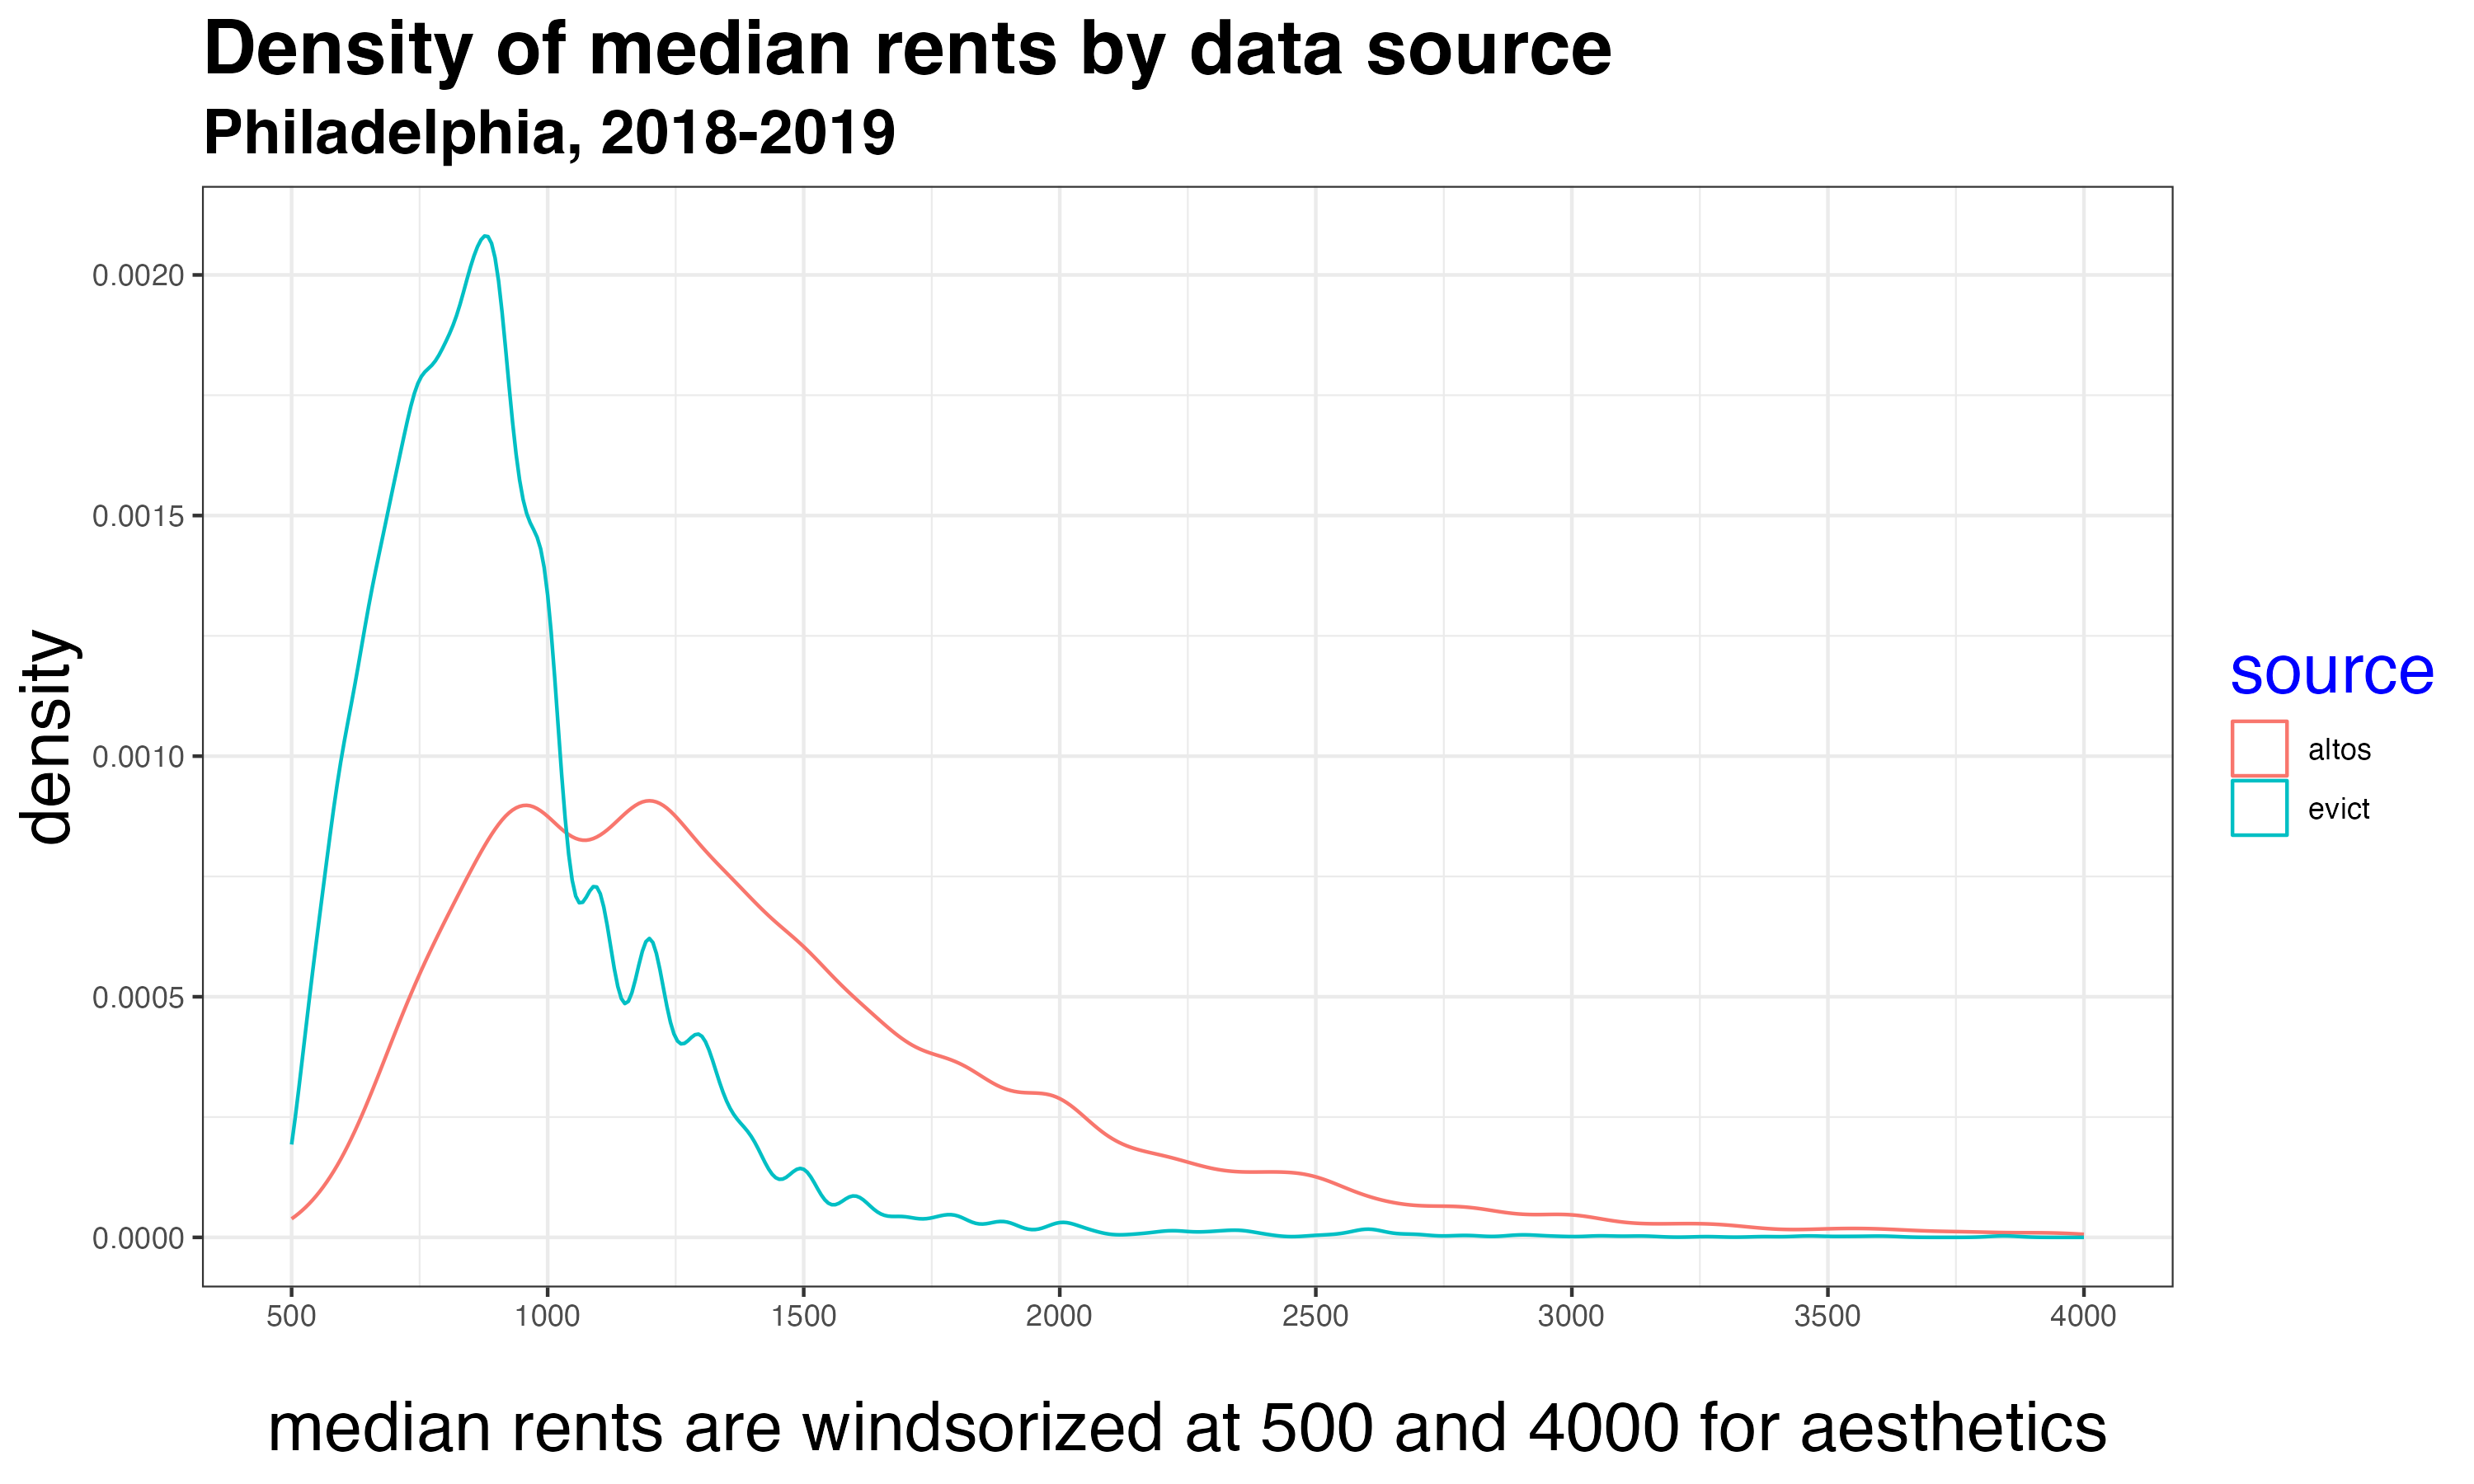
\includegraphics[width=0.75\linewidth]{figs/density_rent_prices.png}
        \caption{Rent Prices by Data Source}
        \label{fig:rent-dist}
    \end{figure}
\end{frame}

\section{Setting and Context}
\begin{frame}{Common Ways of Regulating Eviction}
    \textbf{Filing Fees}
    \begin{itemize}
        \item Increase marginal cost of filing eviction
    \end{itemize}
    \textbf{Right to Counsel}
    \begin{itemize}
        \item Decreases probability of winning an eviction case, conditional on filing; increases amount of time tenant can stay in unit following default; decreases amount tenant pays to landlord
    \end{itemize}
    \textbf{Longer notice periods}
    \textbf{General Legal Climate}
    \begin{itemize}
        \item Good cause eviction ordinances
        \item Restrictions on landlord exit
        \item Allowable reasons for tenants to withhold rent
    \end{itemize}
    
    
\end{frame}

\begin{frame}{Stylized Facts on Eviction in Philadelphia}
    \begin{itemize}
        \item Eviction is relatively infrequent
        \item A small share of properties have very high eviction rates
    \end{itemize}

    \begin{figure}
        \centering
        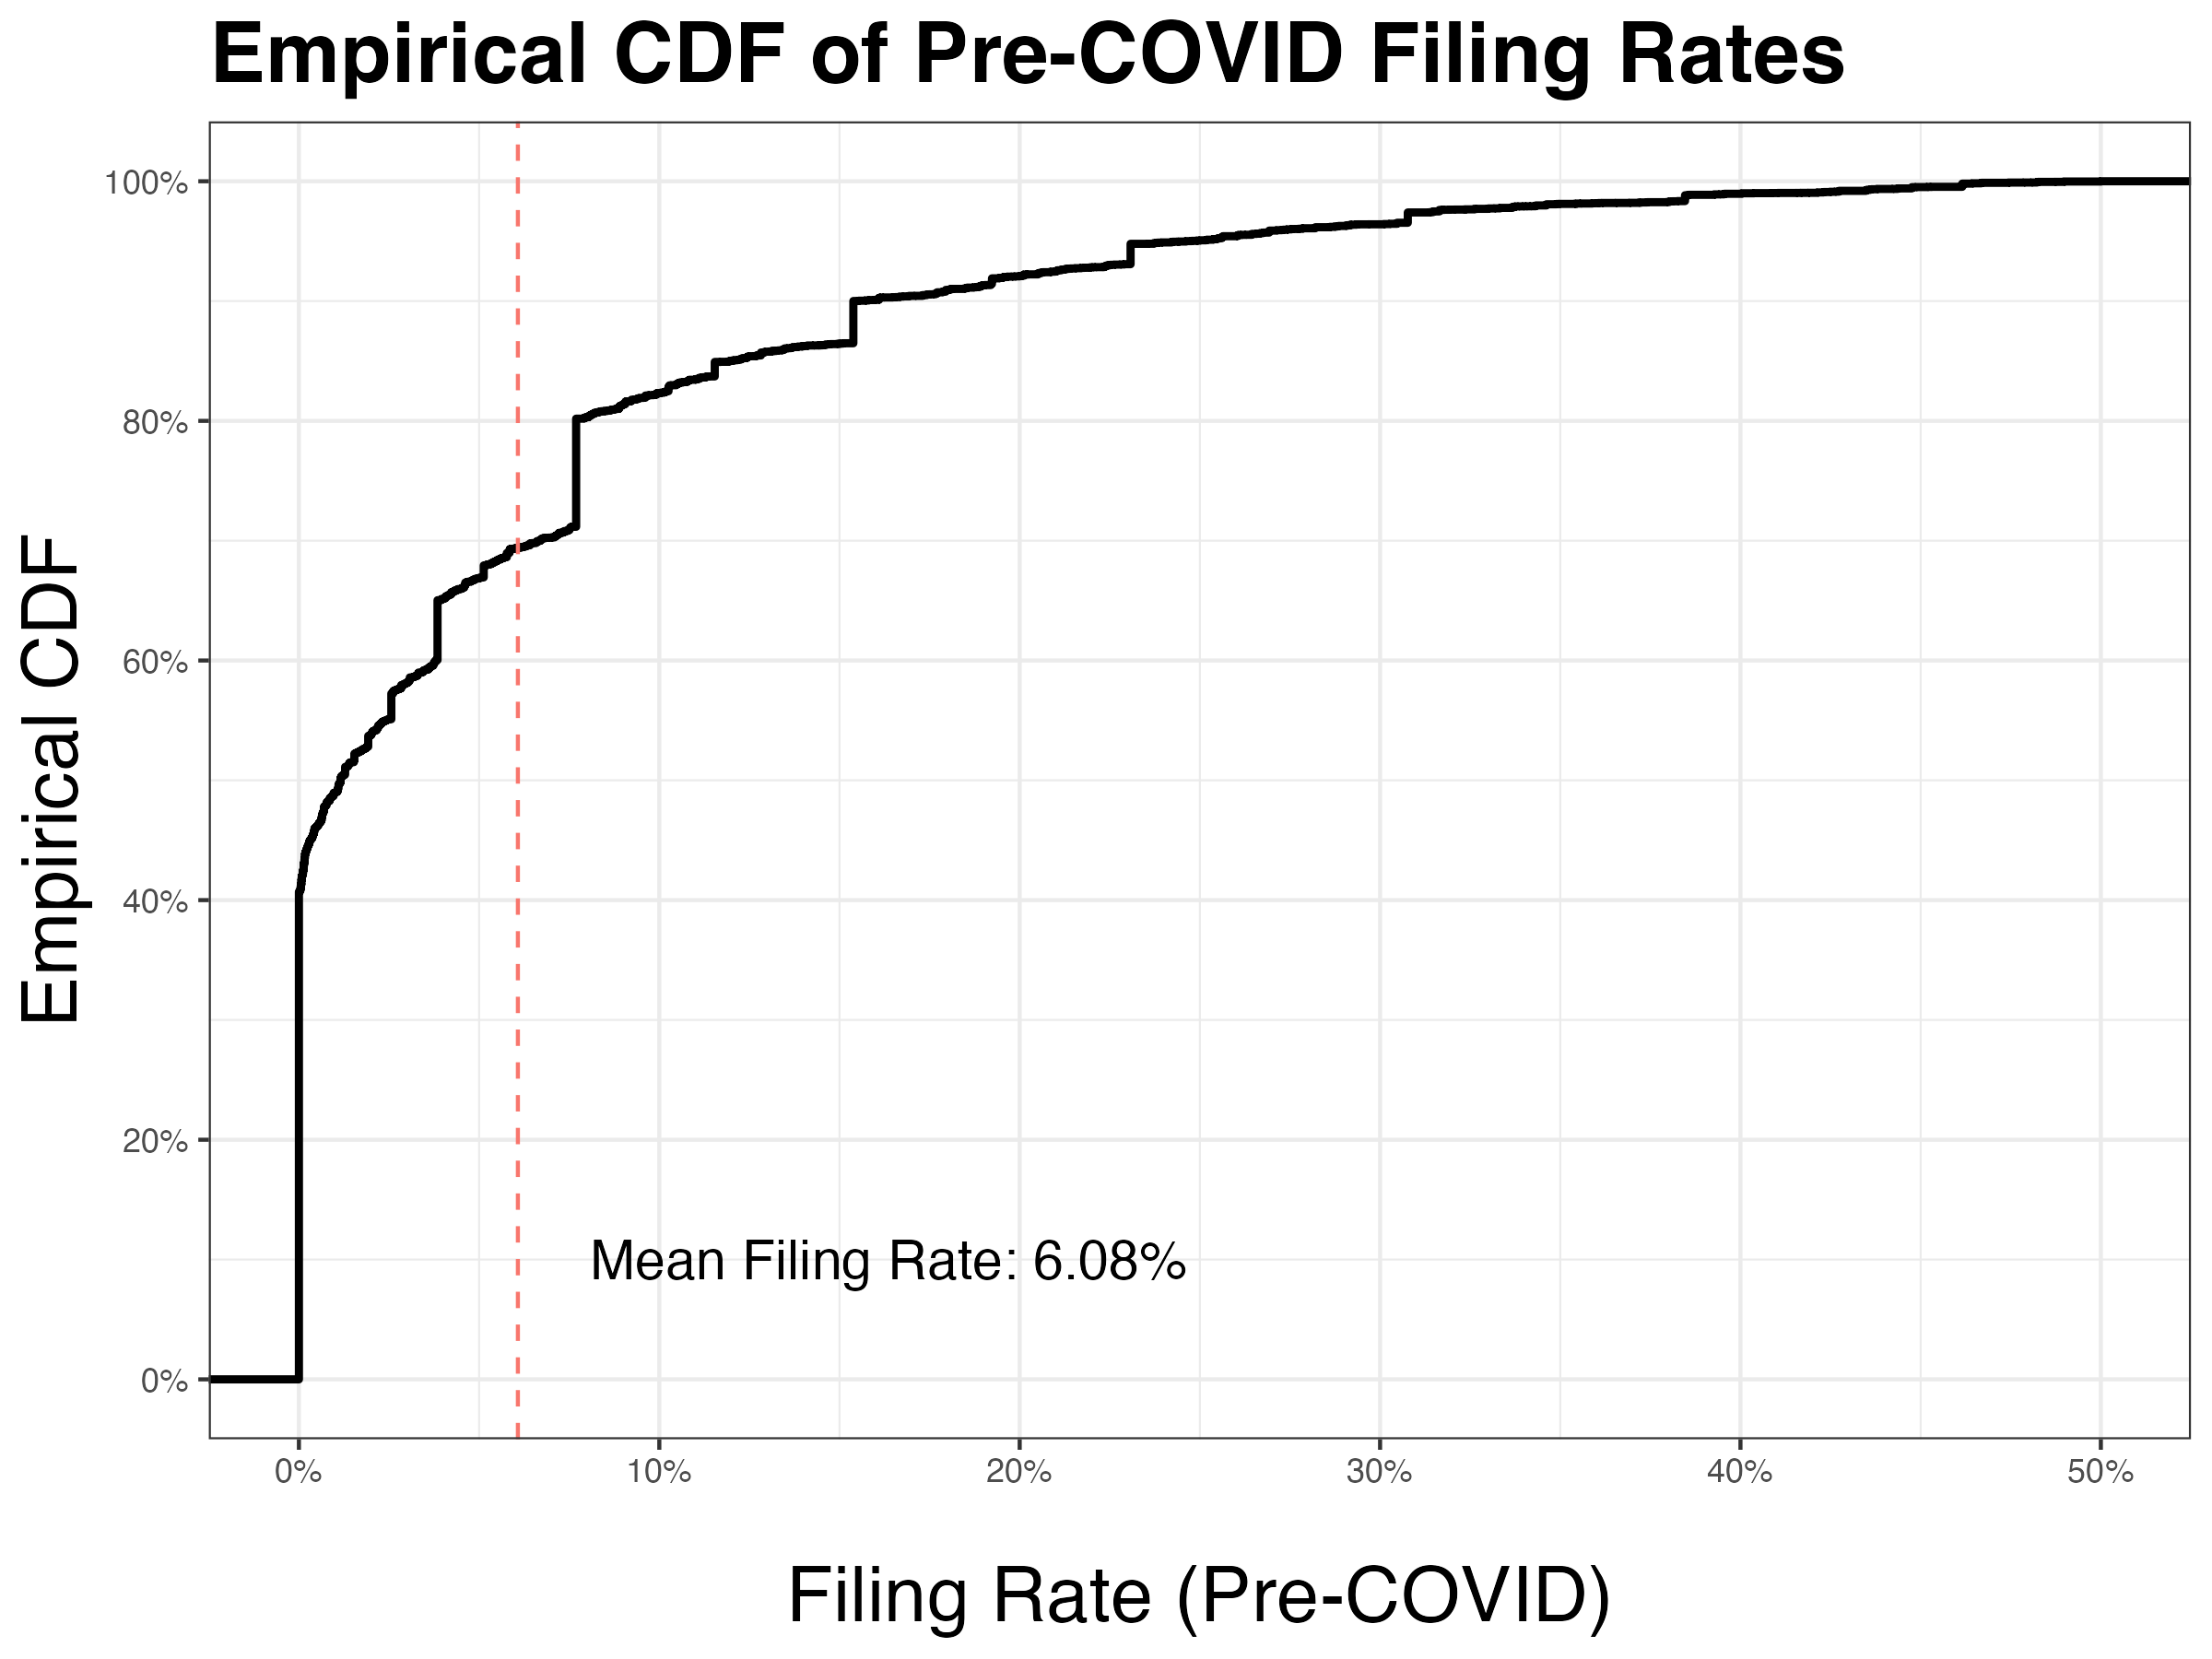
\includegraphics[width=0.75\linewidth]{figs/empirical_cdf_filing_rate_preCOVID.png}
        \caption{Empirical CDF of Filing Rate (pre-COVID)}
        \label{fig:ecdf-filings}
    \end{figure}
    
\end{frame}

\begin{frame}{Evictions in Philadelphia}
    \begin{figure}
        \centering
        \includegraphics[width=0.5\linewidth]{figs/pa_}
        \caption{Caption}
        \label{fig:placeholder}
    \end{figure}
\end{frame}


\begin{frame}{Philadelphia's Eviction Diversion Program}
    \begin{itemize}
        \item Law required all landlords to apply and be approved for the Eviction Diversion Program and participate in good faith for at least 30 days before filing an eviction in court
        \item Depending on the application, the landlord either bargains directly with the tenant or with a tenant and a mediator
        \item if bargaining breaks down, landlord can file an eviction and proceed to court
    \end{itemize}

    Eviction diversion raises the cost of filing an eviction, but can lower the cost of removing a tenant (anecdotally, landlords report higher overall costs). On the tenants' side, eviction diversion prevents an eviction from appearing on their record.
\end{frame}

\begin{frame}{Effectiveness of Philadelphia's Eviction Diversion Program}
    \begin{figure}
        \centering
        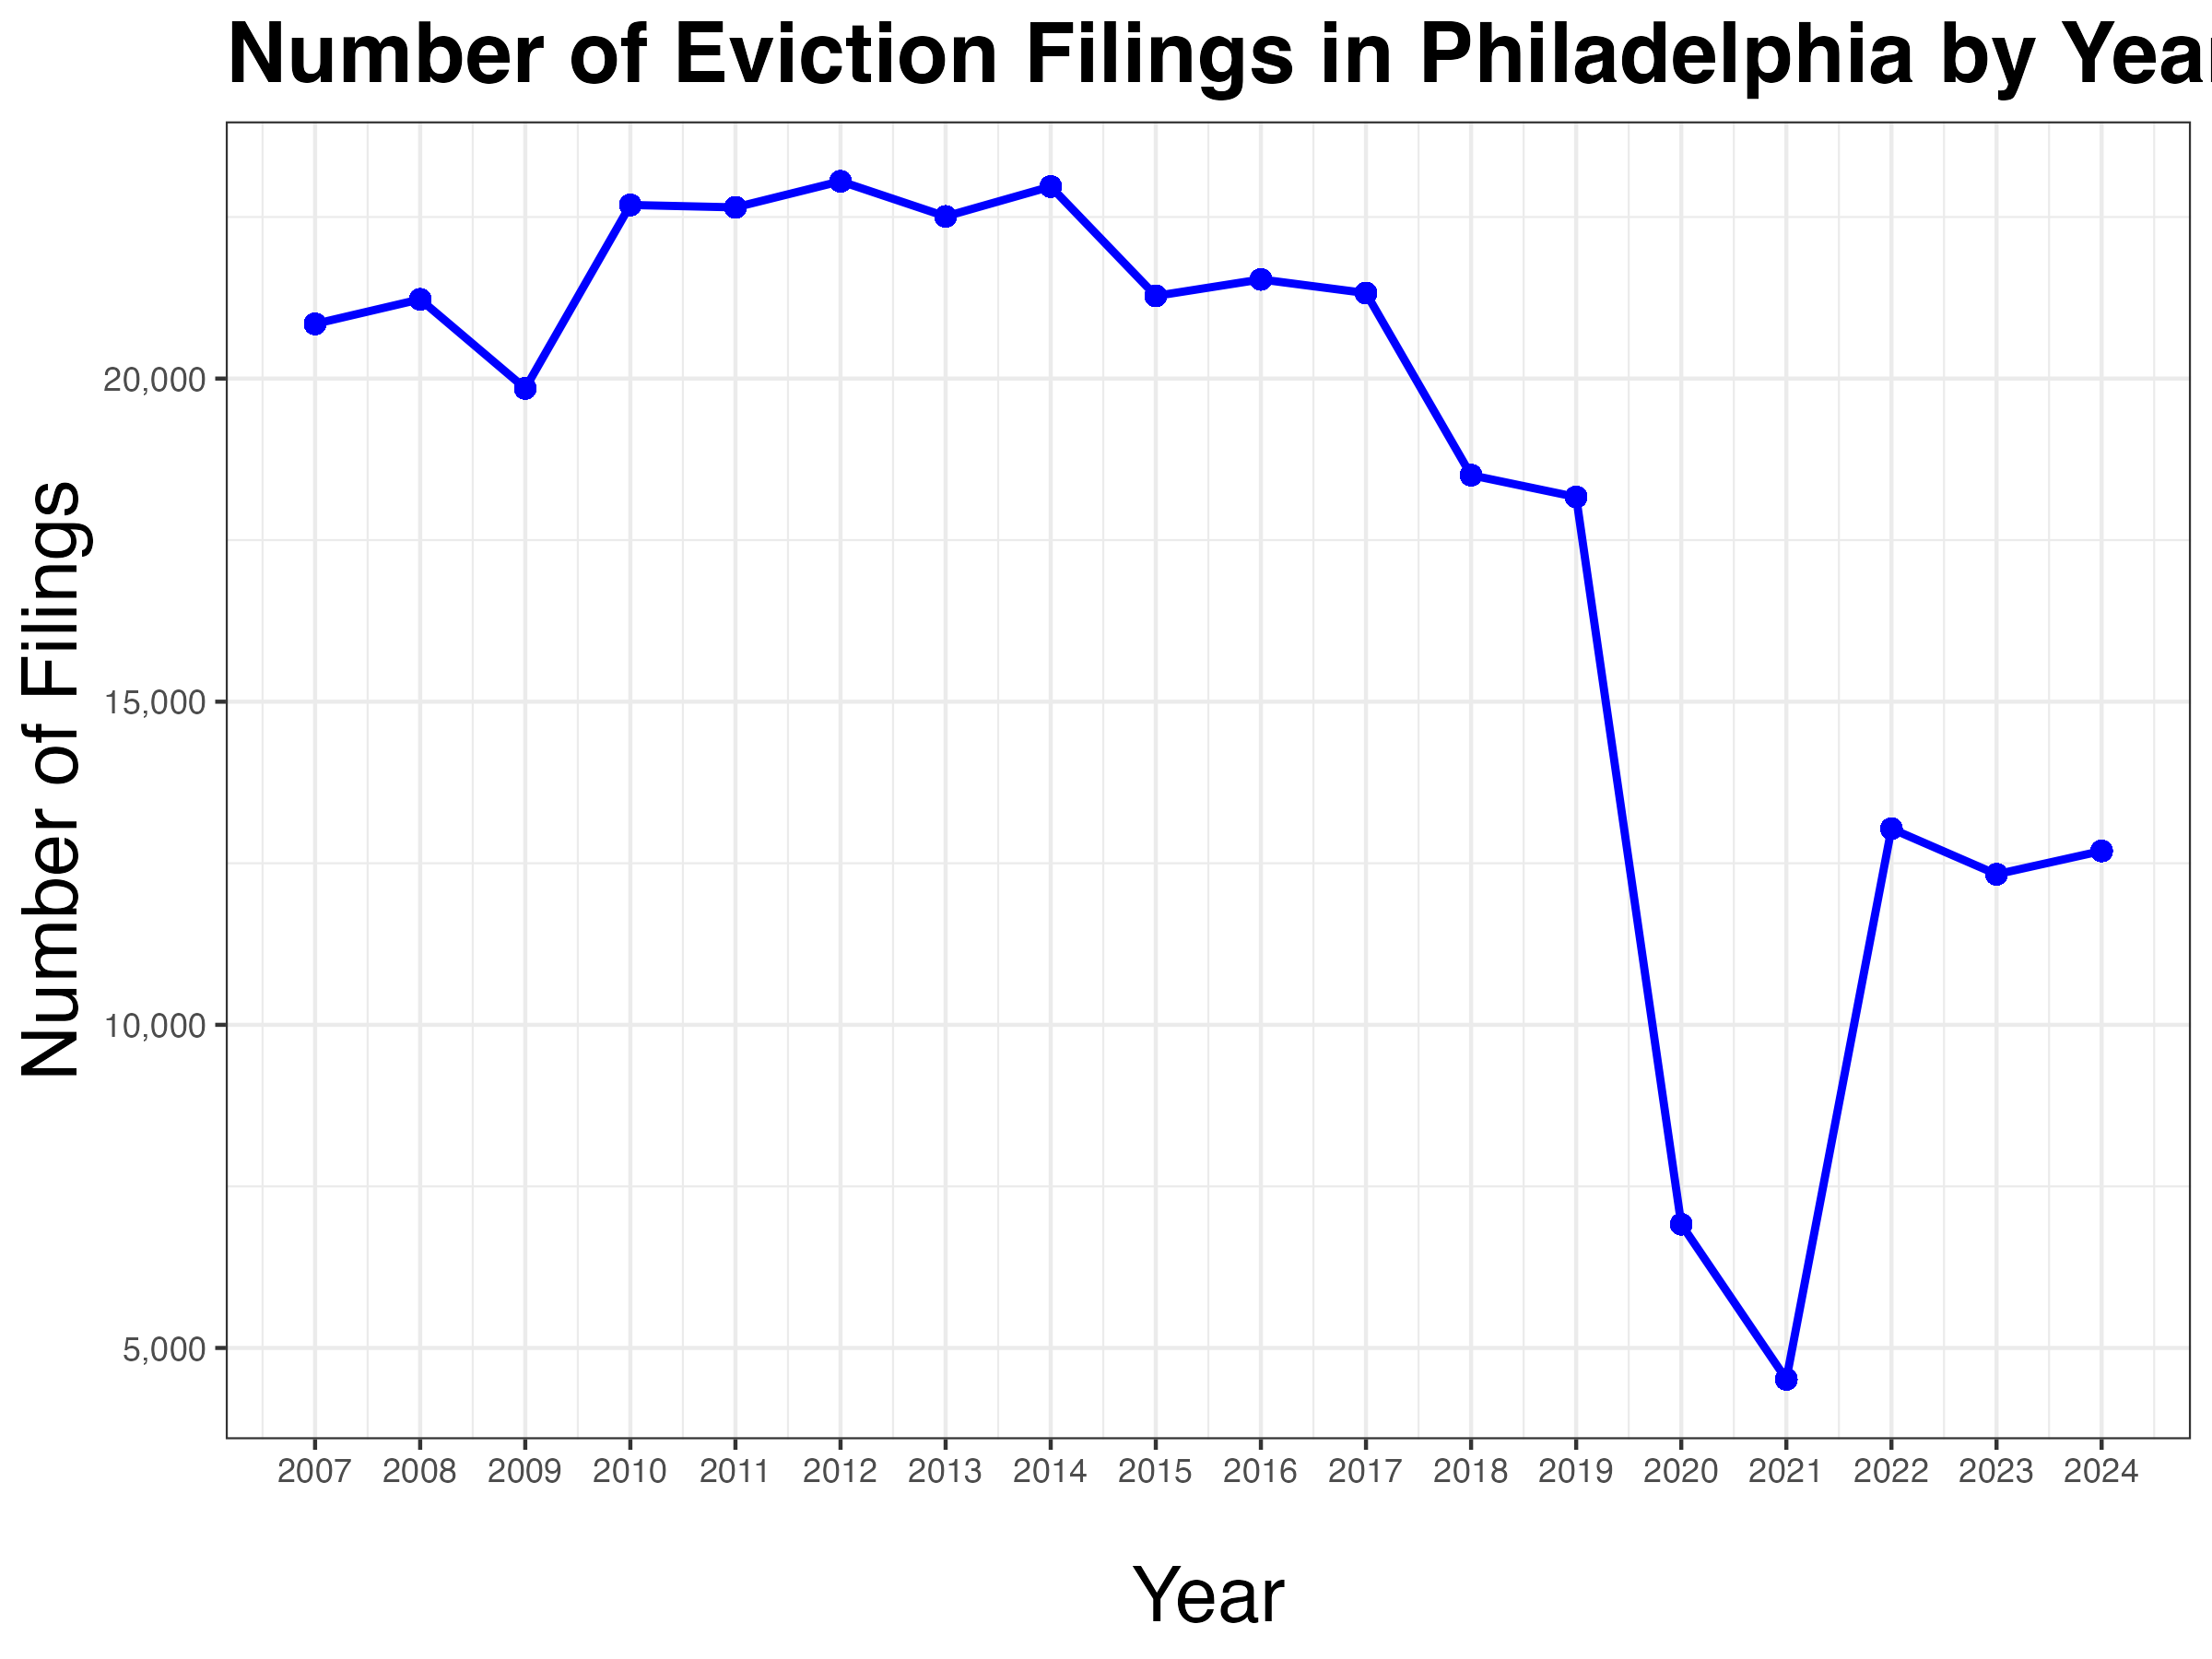
\includegraphics[width=0.75\linewidth]{figs/num_eviction_filings_by_year.png}
        \caption{Eviction Filings by Year}
        \label{fig:evict-year}
    \end{figure}
\end{frame}

\begin{frame}{Changes in landlord response by unit size}
    \begin{figure}
        \centering
        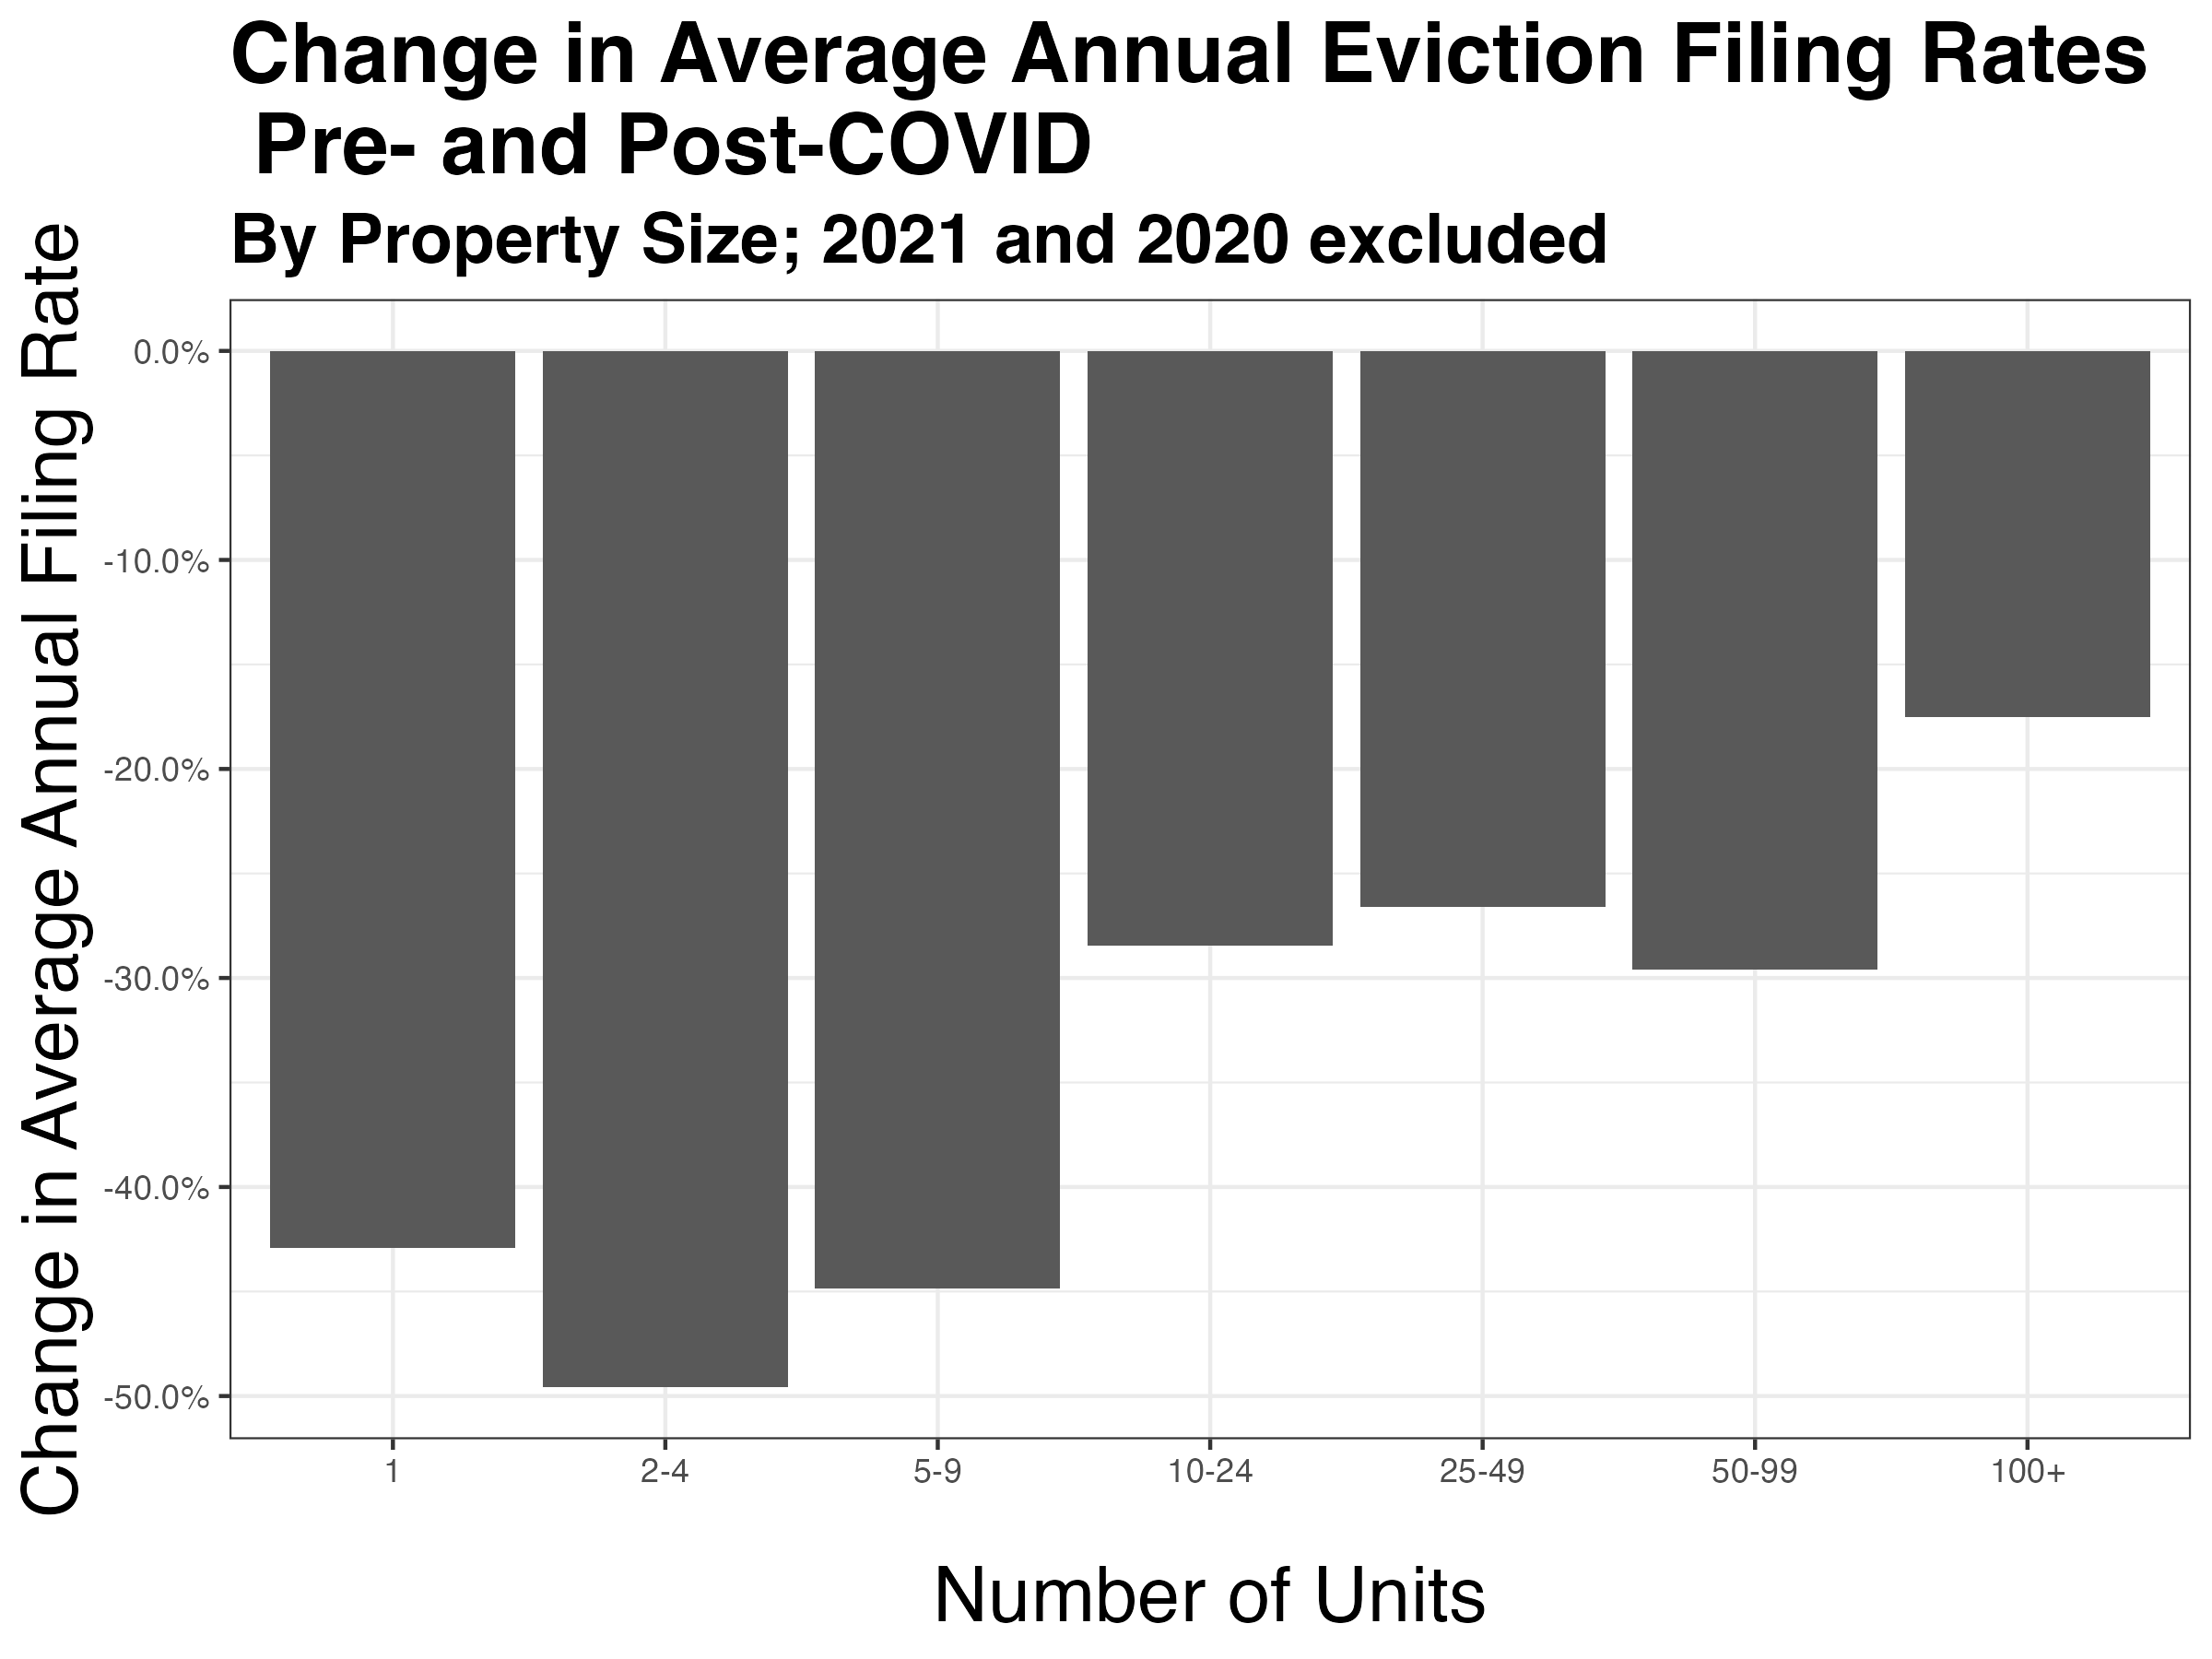
\includegraphics[width=0.75\linewidth]{figs/change_in_avg_annual_eviction_filing_rates_pre_post_COVID_by_num_units.png}
        \caption{Change in filing behavior by number of units}
        \label{fig:change-evict-units}
    \end{figure}
\end{frame}

\begin{frame}{Evidence of Price Effects}
    \begin{figure}
        \centering
        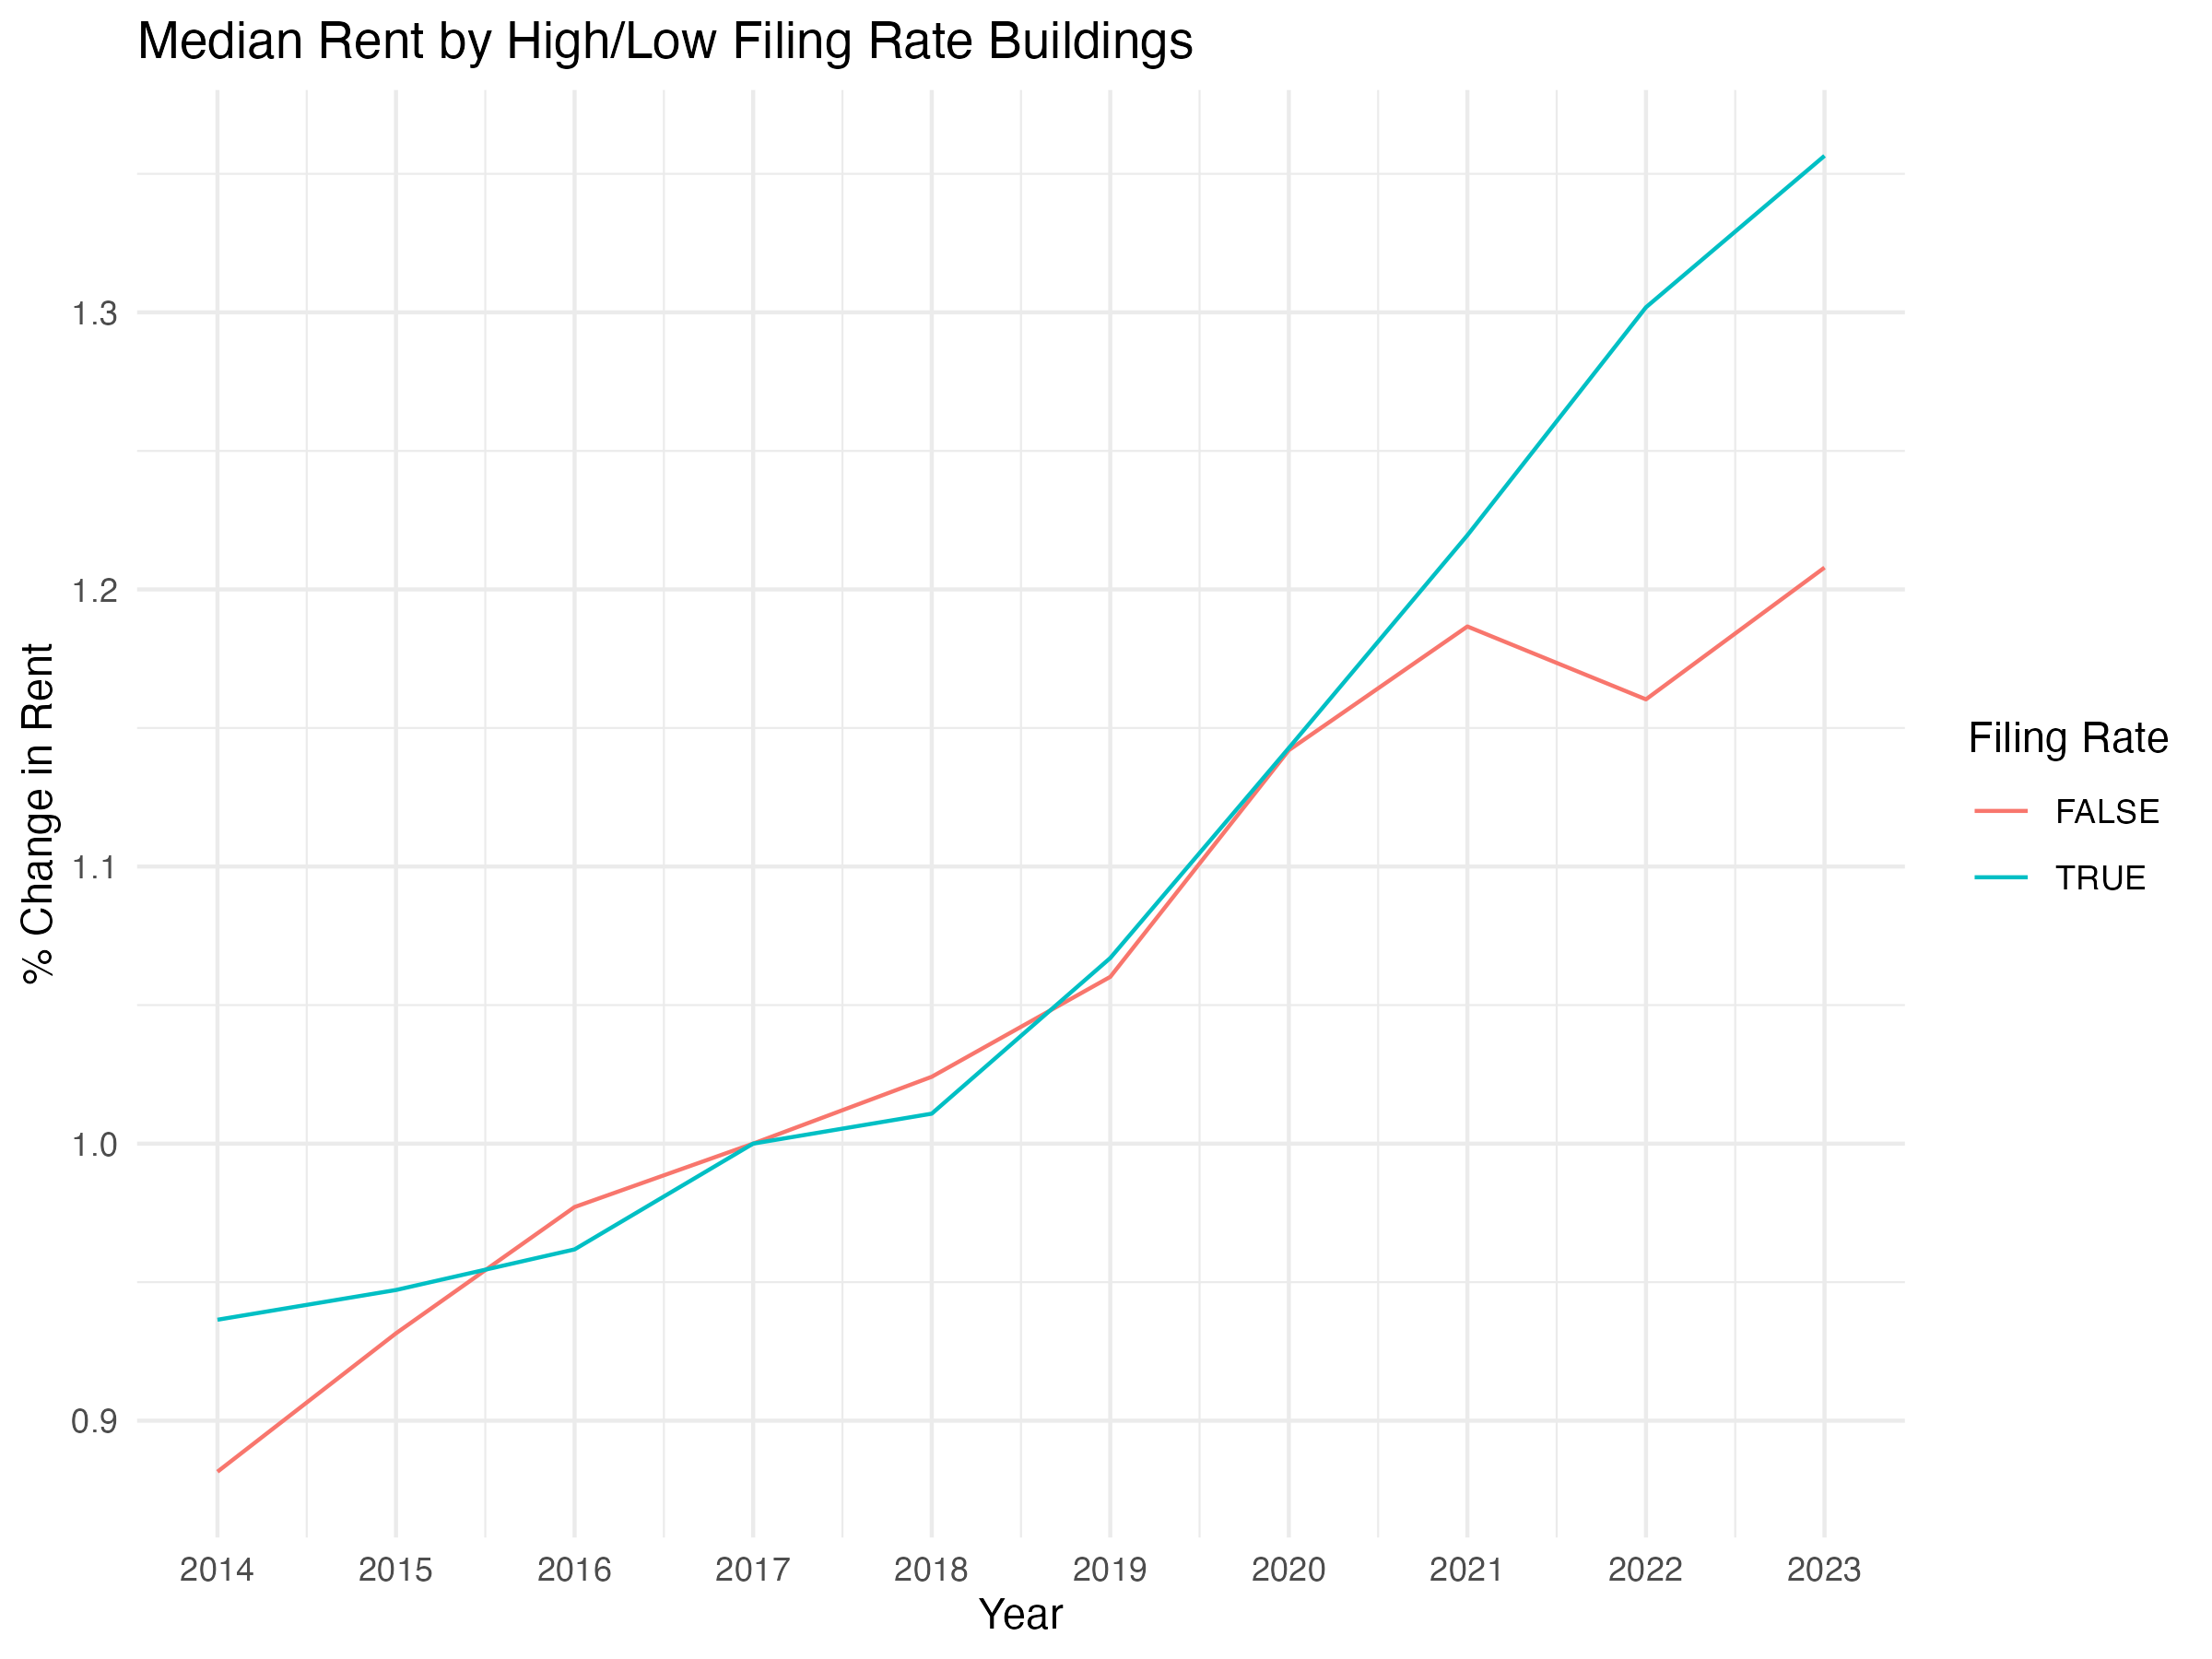
\includegraphics[width=0.5\linewidth]{figs/mean_price_quintile.png}
        \caption{Price Changes over Time}
        \label{fig:price-high-filing}
    \end{figure}
    
\end{frame}

\begin{frame}{High Level Motivation of Model}
\begin{itemize}
    \item Goal is to change landlord conduct (reduce evictions) while inducing minimal pass-through onto rents
    \item The key will be that certain landlords will be closer/farther away from exit/quality upgrading/deferred maintenance 
    \item Papers in the literature \cite{diamond-2019, collinson2024eviction, } all rely on an exit mechanism to move prices; I follow their lead
    \begin{itemize}
        \item Exit is typically condo conversion, so is better thought of as (extreme) quality upgrading
    \end{itemize}
\end{itemize}
    
\end{frame}


% \begin{frame}{Variation in landlord exit opportunities}
%     - put a picture of two high evicting properties
% \end{frame}


\begin{frame}{Toy Model}

\textbf{Model Primitives}
\begin{itemize}
    \item Discount rate $\delta \in (0,1]$
    \item Exogenous initial continuum of landlords $i \in [0,1]$ that each produce one unit of housing
    \item Inverse market demand in Period 2: $P(Q); P'(.) < 0$
    \item Landlord profits = $P(Q) - c_i$
\end{itemize}

\textbf{Timing and Environment}
Two period model. Cost shock happens between time 1 and 2.
\begin{itemize}
    \item At t=1, landlord draws a cost $c_i>0$ and a scrap value $s_i>0$ from a joint CDF $F(c,s)$ with correlation = $\rho$
    \item if the landlord exits at t=1, they get the scrap value $s_i$ immediately; if they stay, they get flow profit = $P(Q) - c_i$
\end{itemize}


\end{frame}

\begin{frame}{Toy Model Continued}
\textbf{Landlord Problem}
Landlord stays in the market iff
\begin{align*}
    \delta(P(Q) - c_i) \geq s_i
\end{align*}

Define S(p) as the set of all prices such that a landlord continues for a given $c,s$
\begin{align*}
    S(p) & = \big\{(c,s): c \leq p, s \leq \delta(p - c)
\end{align*}

Then supply is equal to 
\begin{align*}
    S(P) =  \int\int_{S(P)}dF(c,s)
\end{align*}

Markets clear such that $p*$ solves $D(p*) = S(p*)$


    
\end{frame}

\begin{frame}{Toy Model Comparative Statics}
For a given price, a higher $\rho$ shifts out the set of landlords who will exit, so $S(P)$ increases with $\rho$. Since demand slopes downwards, this means $\frac{dp*}{d\rho} >0$\\

Intuitively, price response will be worse in a world where more marginal landlords are targeted by the cost increase
    
\end{frame}

\begin{frame}{Toy Model Continued}
    In reality, landlords have more options than a simple exit/continue decision:
    - change screening practices
    - quality upgrading
    - immediate exit
    Covariance between adjustment mechanisms and cost increases will be determinant of price hike. Degree of market segmentation will also affect price responses
\end{frame}

\begin{frame}{Toy Model Nested Logit}
    \begin{itemize}
        \item Discount rate $\delta \in (0,1]$
        \item Exogenous initial continuum of landlords $i \in [0,1]$ that each produce one unit of housing
        \item Low nest ($L$) and high nest ($H$); each landlord is active in one nest
        \item Market size $M$ is normalized to $J=n_l +n_h$
        \item At t=1, \textbf{low tier landlords} draw costs $c_i>0$, and a quality upgrading cost $q_i>0$ from a joint CDF $F(c,q)$ with correlation = $\rho'$
        \item \textbf{low tier landlords} can now pay an upgrade cost $q$ to enter the high tier, or continue and make low tier flow profits
    \end{itemize}    
\end{frame}

\begin{frame}{Toy Model Cont.}
    Product $j$ in nest $g(j)$ has mean utility $\delta_j$; price coefficient $\alpha>0$; nest correlation (segmentation) $\sigma\in[0,1)$. \\
    
    Within-nest shares and inclusive values:
        \begin{align*}
            s_{j|g} \;=\;
            \frac{\exp\!\left(\frac{\delta_j-\alpha p_j}{1-\sigma}\right)}
            {\sum_{k\in g}\exp\!\left(\frac{\delta_k-\alpha p_k}{1-\sigma}\right)},
            \qquad
            I_g \;=\; (1-\sigma)\,\log\!\sum_{k\in g}\exp\!\left(\frac{\delta_k-\alpha p_k}{1-\sigma}\right).
        \end{align*}
    Nest shares (no outside):
        \begin{align*}
            S_g \;=\;\frac{e^{I_g}}{e^{I_L}+e^{I_H}},
            \qquad
            s_j \;=\; S_{g(j)}\,s_{j|g(j)},
            \qquad
            S_L+S_H \;=\; 1.
        \end{align*}
    
    \emph{Symmetric-within-nest specialization} (identical products in a nest) implies
        \begin{align*}
            \boxed{\,s_j=\tfrac{1}{J},\;\; s_{j|g}=\tfrac{1}{n_g},\;\; S_g=\tfrac{n_g}{J}\,}.
        \end{align*}
    
\end{frame}

\begin{frame}{Nested Logit Pricing}
    With symmetry in nest $g$ (common price $p_g$), the optimal \emph{per-product markup} is
        \begin{align*}
            p_g - c_g \;=\; \frac{s_j}{\alpha\big[1 - \sigma(1-s_{j|g}) - (1-\sigma)(1-S_g)\big]}.
        \end{align*}
plugging the symmetric shares $s_j=\tfrac{1}{J}$, $s_{j|g}=\tfrac{1}{n_g}$, $S_g=\tfrac{n_g}{J}$ yields the \emph{capacity-consistent} closed form:
\begin{align*}
\boxed{
\,p_g - c_g
\;=\;
\frac{1}{\alpha\,J\Big(1 - \sigma\!\big(1-\tfrac{1}{n_g}\big) - (1-\sigma)\!\big(1-\tfrac{n_g}{J}\big)\Big)}\;,\quad g\in\{L,H\}.
}
\end{align*}
Because $M=J$ and $s_j=1/J$, each seller’s quantity is $1$, so \emph{per-seller operating profit equals the markup}:
\begin{align*}
    \boxed{\,\Pi_g(n_L,n_H) \;=\; p_g - c_g\,}.
\end{align*}
    
\end{frame}

\begin{frame}{Nested Logit Comparative Statics}
    \textbf{Landlord choice (upgrade vs stay in L) with $(\kappa_i,\phi_i)$ correlated.}
Given a draw $(\kappa_i,\phi_i)$:
\begin{align*}
\pi_i^{L} &= p_L - \kappa_i, 
&
\pi_i^{H} &= -\phi_i p_H.
\end{align*}

For simplicity, assume $\pi_h = \pi_l$
\begin{align*}
\boxed{\;\kappa_i  \;\ge\; \phi_i }.
\end{align*}

Now, prices in the low nest, depend on $\rho$ and on the degree of market segmentation $\sigma$

\end{frame}

\section{Evidence of Market Segmentation}

\begin{frame}{Evidence of Market Segmentation}
    
\end{frame}

\begin{frame}{Evidence of Market Segmentation: Cont.}
    put table with gravity eq about here
\end{frame}

\begin{frame}{Evidence of Market Segmentation: Nested Logit}
    
\end{frame}

\begin{frame}{Nested Logit Results}
    
\end{frame}

\begin{frame}{Evidence of Market Segmentation: Nested Logit}
\end{frame}

% \begin{frame}{Landlord Behavior post-COVID}
    
% \end{frame}

% \begin{frame}{Landlord Exit / Entry Model}
    
% \end{frame}

% \begin{frame}{Landlord Exit / Entry Model: Calibration}
    
% \end{frame}

% \begin{frame}{Landlord Exit / Entry Model: Counterfactual}
    
% \end{frame}
    




\end{document}
